Maintenant que nous savons comment les Subtrees sont créés, il ne reste plus qu'à savoir les transmettre au client Cesium. Ce client accepte sous deux formats différents. Nous pouvons soit lui envoyer la description du Subtree sous forme de JSON et lui envoyer les listes de disponibilités dans des fichiers binaires séparément en précisant les URI de ces fichiers dans le JSON. Comme seconde option, nous pouvons tout lui envoyer en un seul fichier binaire qui respecte le \href{https://github.com/CesiumGS/3d-tiles/tree/main/specification/ImplicitTiling#subtree-binary-format}{\textit{Subtree Binary Format}}\footnote{https://github.com/CesiumGS/3d-tiles/tree/main/specification/ImplicitTiling\#subtree-binary-format}. Sous ce format, les fichiers binaires sont inclus sous forme de buffer binaire. Les différentes listes de disponibilités pourront ensuite être retrouvées grâce à des offsets indiqués dans la partie JSON à la place des URI. Sauf raison externe, cette deuxième option est généralement plus simple à utiliser. C'est pourquoi je l'ai choisie pour mon implémentation.

Le \textit{Subtree Binary Format} est un format où les informations sont stockées en little-endian et dont les fichiers comportent un header de 24 Bytes. Ce header contient les informations suivantes :

\begin{figure}[H]
    \centering
    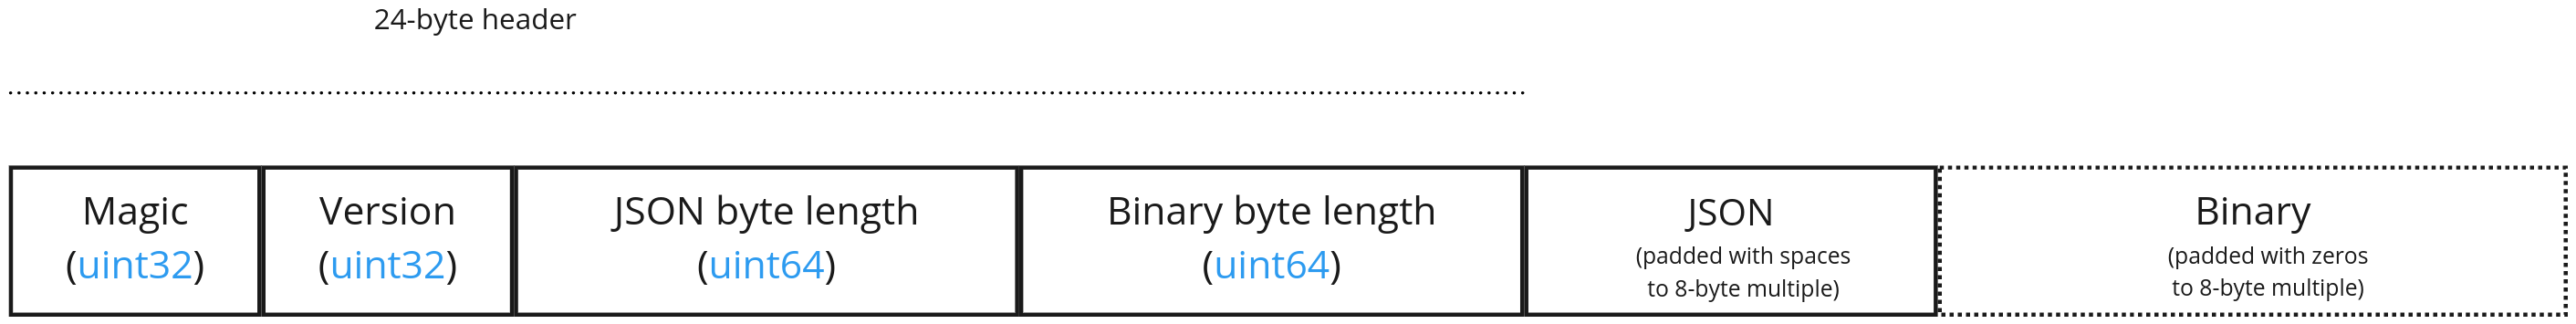
\includegraphics[width=1\textwidth]{assets/figures/binary-subtree.png}
    \caption{Header d'un fichier au \textit{Subtree Binary Format} \cite{implicit-tiling-gh}}
    \label{fig:xy-morton}
\end{figure}

Les informations contenues dans le header sont les suivantes :

\begin{itemize}
    \item \textbf{Magic} : 4 Bytes, \textit{magic number} identifiant ce fichier comme un Subtree. A toujours une valeur de \texttt{0x74627573}.
    \item \textbf{Version} : 4 Bytes, version du format binaire. Actuellement, le 24.07.2024, il s'agit de 1.
    \item \textbf{JSON Byte Length} : 8 Bytes, longueur de la partie JSON en Bytes.
    \item \textbf{Binary Byte Length} : 8 Bytes, longueur de la partie binaire en Bytes.
\end{itemize}

Concernant le \href{https://www.lalanguefrancaise.com/dictionnaire/definition/padding}\textit{padding}\footnote{https://www.lalanguefrancaise.com/dictionnaire/definition/padding}, les deux derniers éléments, \textit{JSON Byte Length} et \textit{Binary Byte Length}, doivent compter les Bytes de padding. Le padding est nécessaire car chaque chunk doit être aligné sur une frontière de 8 Bytes. La partie doit être remplie avec le caractère espace (\texttt{0x20}) sur la fin, tandis que la partie binaire doit être remplie avec des zéros (\texttt{0x00}) sur la fin.

\newpage
\subsection{Écriture de JSON}

Le JSON doit contenir les objets suivants :

\begin{itemize}
    \item \textbf{buffers} : une liste d'objet contenant le nom, les URI si nécessaire et la longueur des buffers binaires.
    \item \textbf{bufferViews} : une liste d'objet contenant les les offsets des différentes parties des buffers binaires.
    \item \textbf{tileAvailability} : un objet décrivant liste de disponibilités des tuiles.
    \item \textbf{contentAvailability} : un objet décrivant liste de disponibilités des contenus.
    \item \textbf{childAvailability} : un objet décrivant liste de disponibilités des enfants.
\end{itemize}

Les objets \texttt{buffer} doivent contenir les informations suivantes :

\begin{itemize}
    \item \textbf{name} : nom du buffer.
    \item \textbf{uri} : URI du fichier binaire, doit être omis si on utilise le \textit{Subtree Binary Format}.
    \item \textbf{byteLength} : longueur du fichier binaire.
\end{itemize}

Les objets \texttt{bufferViews} doivent contenir les informations suivantes :

\begin{itemize}
    \item \textbf{buffer} : index du buffer auquel le bufferView fait référence dans la liste de buffers.
    \item \textbf{byteOffset} : offset de la vue dans le buffer.
    \item \textbf{byteLength} : longueur de la vue.
\end{itemize}

Les objets \texttt{tileAvailability}, \texttt{contentAvailability} et \texttt{childAvailability} peuvent soit contenir un objet \texttt{constant} ayant une valeur de \texttt{0} ou \texttt{1} qui signifie que toutes les tuiles ont la même disponibilité. Soit contenir un objet \texttt{bufferView} qui fait référence à un bufferView contenant les listes de disponibilités avec un objet \texttt{availableCount} qui indique le nombre de tuiles disponibles.

\begin{itemize}
    \item \textbf{constant} : objet contenant une valeur de \texttt{0} ou \texttt{1}.
    \item \textbf{bufferView} : index du bufferView contenant les listes de disponibilités.
    \item \textbf{availableCount} : nombre de tuiles disponibles.
\end{itemize}

D'autres informations peuvent notamment être ajoutées au JSON tel que des metadata.

Voici un exemple de JSON d'un des Subtrees créés par mon implémentation :

\begin{verbatim}
    TODO
\end{verbatim}